\documentclass[a4paper,12pt]{jarticle}
\usepackage[dvipdfmx]{graphicx}
\usepackage{amsmath}
\usepackage{subfigure}
\usepackage{comment}
\usepackage{array}


\setlength{\hoffset}{0cm}
\setlength{\oddsidemargin}{-3mm}
\setlength{\evensidemargin}{-3cm}
\setlength{\marginparsep}{0cm}
\setlength{\marginparwidth}{0cm}
\setlength{\textheight}{24.7cm}
\setlength{\textwidth}{17cm}
\setlength{\topmargin}{-45pt}

\renewcommand{\baselinestretch}{1.6}
\renewcommand{\floatpagefraction}{1}
\renewcommand{\topfraction}{1}
\renewcommand{\bottomfraction}{1}
\renewcommand{\textfraction}{0}
\renewcommand{\labelenumi}{(\arabic{enumi})}
%\renewcommand{\figurename}{Fig.} %図をFig.にする


%図のキャプションからコロン:を消す
\makeatletter
\long\def\@makecaption#1#2{% #1=図表番号、#2=キャプション本文
\sbox\@tempboxa{#1. #2}
\ifdim \wd\@tempboxa >\hsize
#1 #2\par 
\else
\hb@xt@\hsize{\hfil\box\@tempboxa\hfil}
\fi}
\makeatother


\begin{document}
%
\title{\vspace{-30mm}知能システム学特論 \ 最終レポート\\ Hdp第2班 16344217 津上祐典\\ 2016年8月19日}
\date{}
%
%
\maketitle
%
\vspace{-30mm}
%
%%%%%%%%%%%%%%%%%%%
 \section{テーマ}
%%%%%%%%%%%%%%%%%%
SparkとHadoopを用いた分散機械学習によるクラス分類 -スパムメールの検出と
画像認識
%%%%%%%%%%%%%%%%%%%
\section{概要}
%%%%%%%%%%%%%%%%%%%
はじめに,Hadoop,Spark,機械学習の原理ついて述べ,最後に実行結果と考察を
示す.
%%%%%%%%%%%%%%%%%%%%%%%
\subsection{Hadoop}
%%%%%%%%%%%%%%%%%%%%%%%
Hadoopとはビッグデータを複数のPCを用いて分散並列処理を可能にするフレームワークであ
る.ー台マスターサーバとその配下にある複数のスレーブサーバによって分散
並列処理を行う.
Hadoopは分散ファイルシステム(Hadoop Distributed File
System),並列分散処理フレームワーク(MapReduce
Framework)より構成されている.Hadoopの構成を図\ref{fig:hadoop}に示す.
分散ファイルシステムとは複数のスレーブサーバを一つのストレー
ジとして扱うファイルシステムである.
分散並列処理フレームワークでは与えられたデー
タから欲しいデータの抽出と分解するMap処理,それらのデータを集計する
Reduce処理が行われる.MapReduce処理を複数のスレーブサーバで行うことで分
散処理を可能にし,ビッグデータを効率よく扱うことができる.
図\ref{fig:MapReduce}にHadoopの分散処理の流れを示す.Hadoopの分散処理は
以下の流れで行う;1) HDFSよりデータを分割し,各スレーブサーバへ入力デー
タとして入る,2) 入力されたデータから欲しいデータを抽出し,分解する(Map
処理),3) 各スレーブサーバでMap処理が行われたデータを整理する(Shuffle),
4) 整理させたデータを集計し,結果を出力する(Reduce処理).
%
\begin{figure}[htbp]
 \begin{center}
  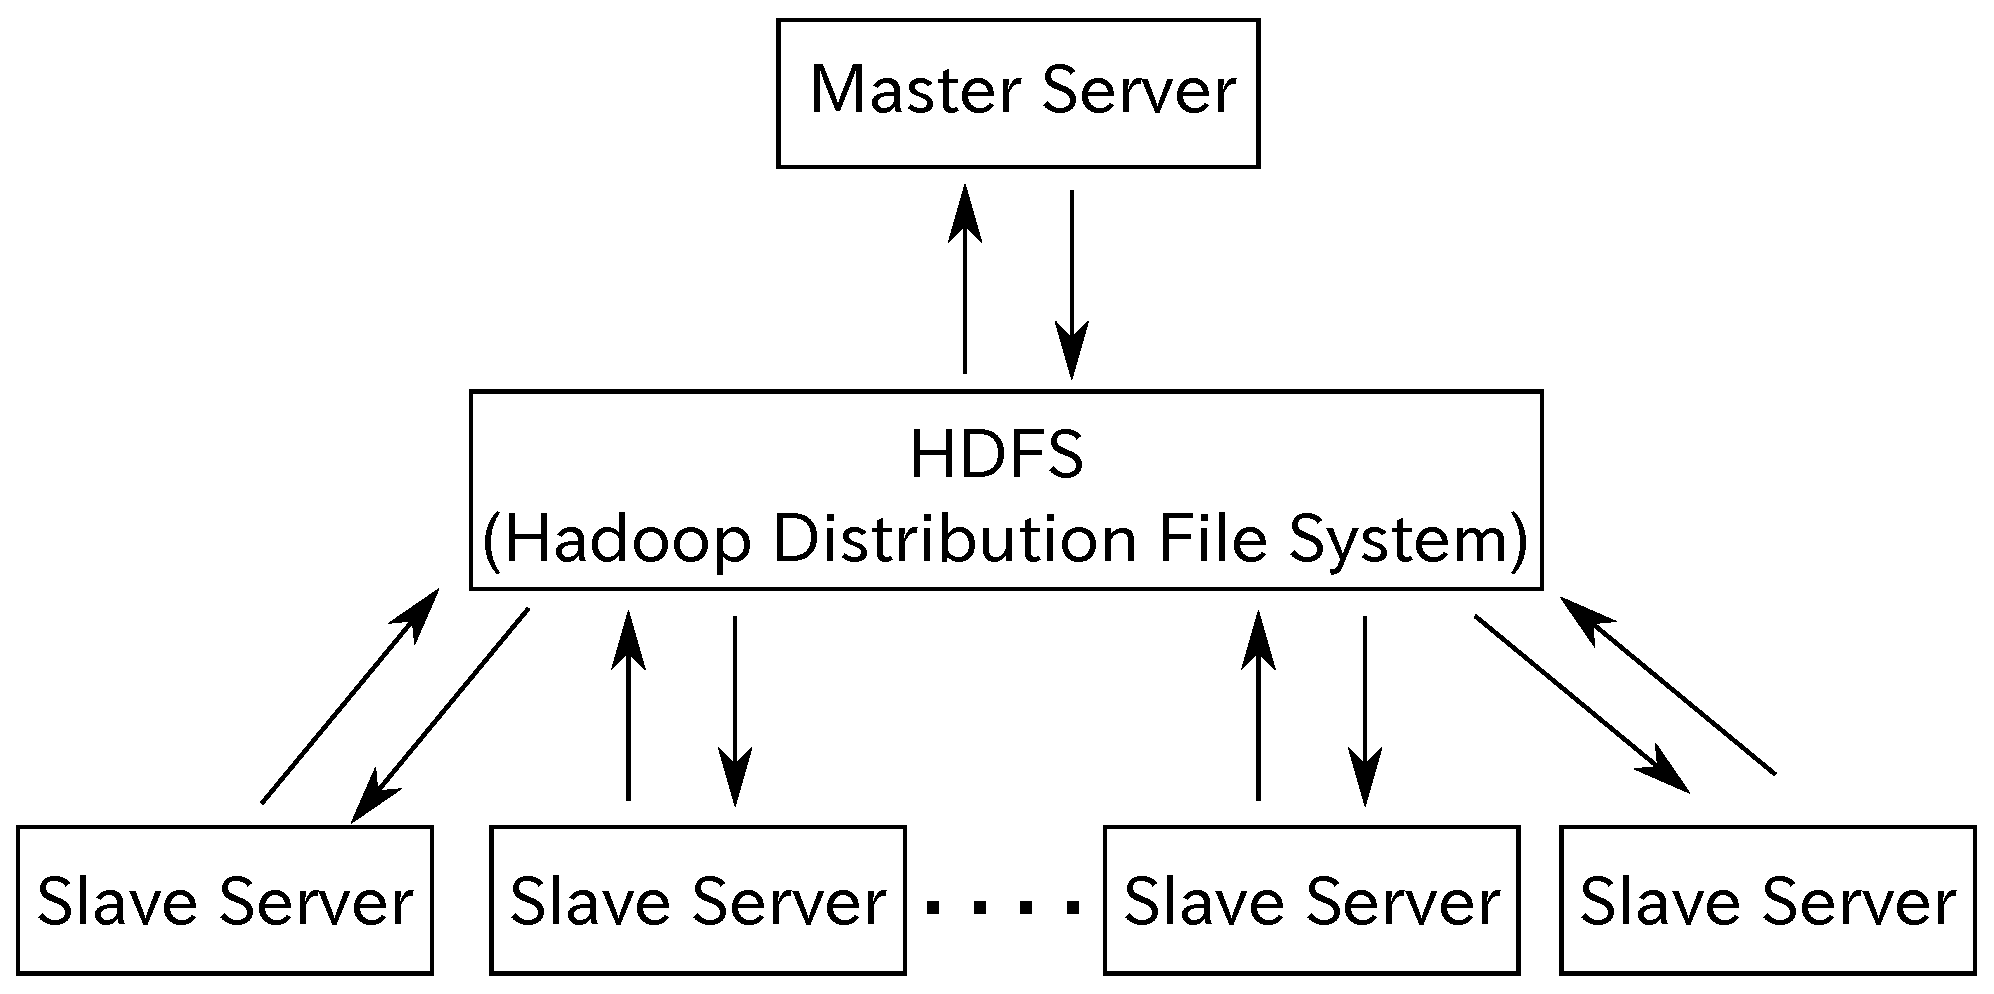
\includegraphics[width=100mm]{fig/Hadoop.eps}
  \caption{Hadoopの構成}
  \label{fig:hadoop}
 \end{center}
\end{figure}
%
%
\begin{figure}[htbp]
 \begin{center}
  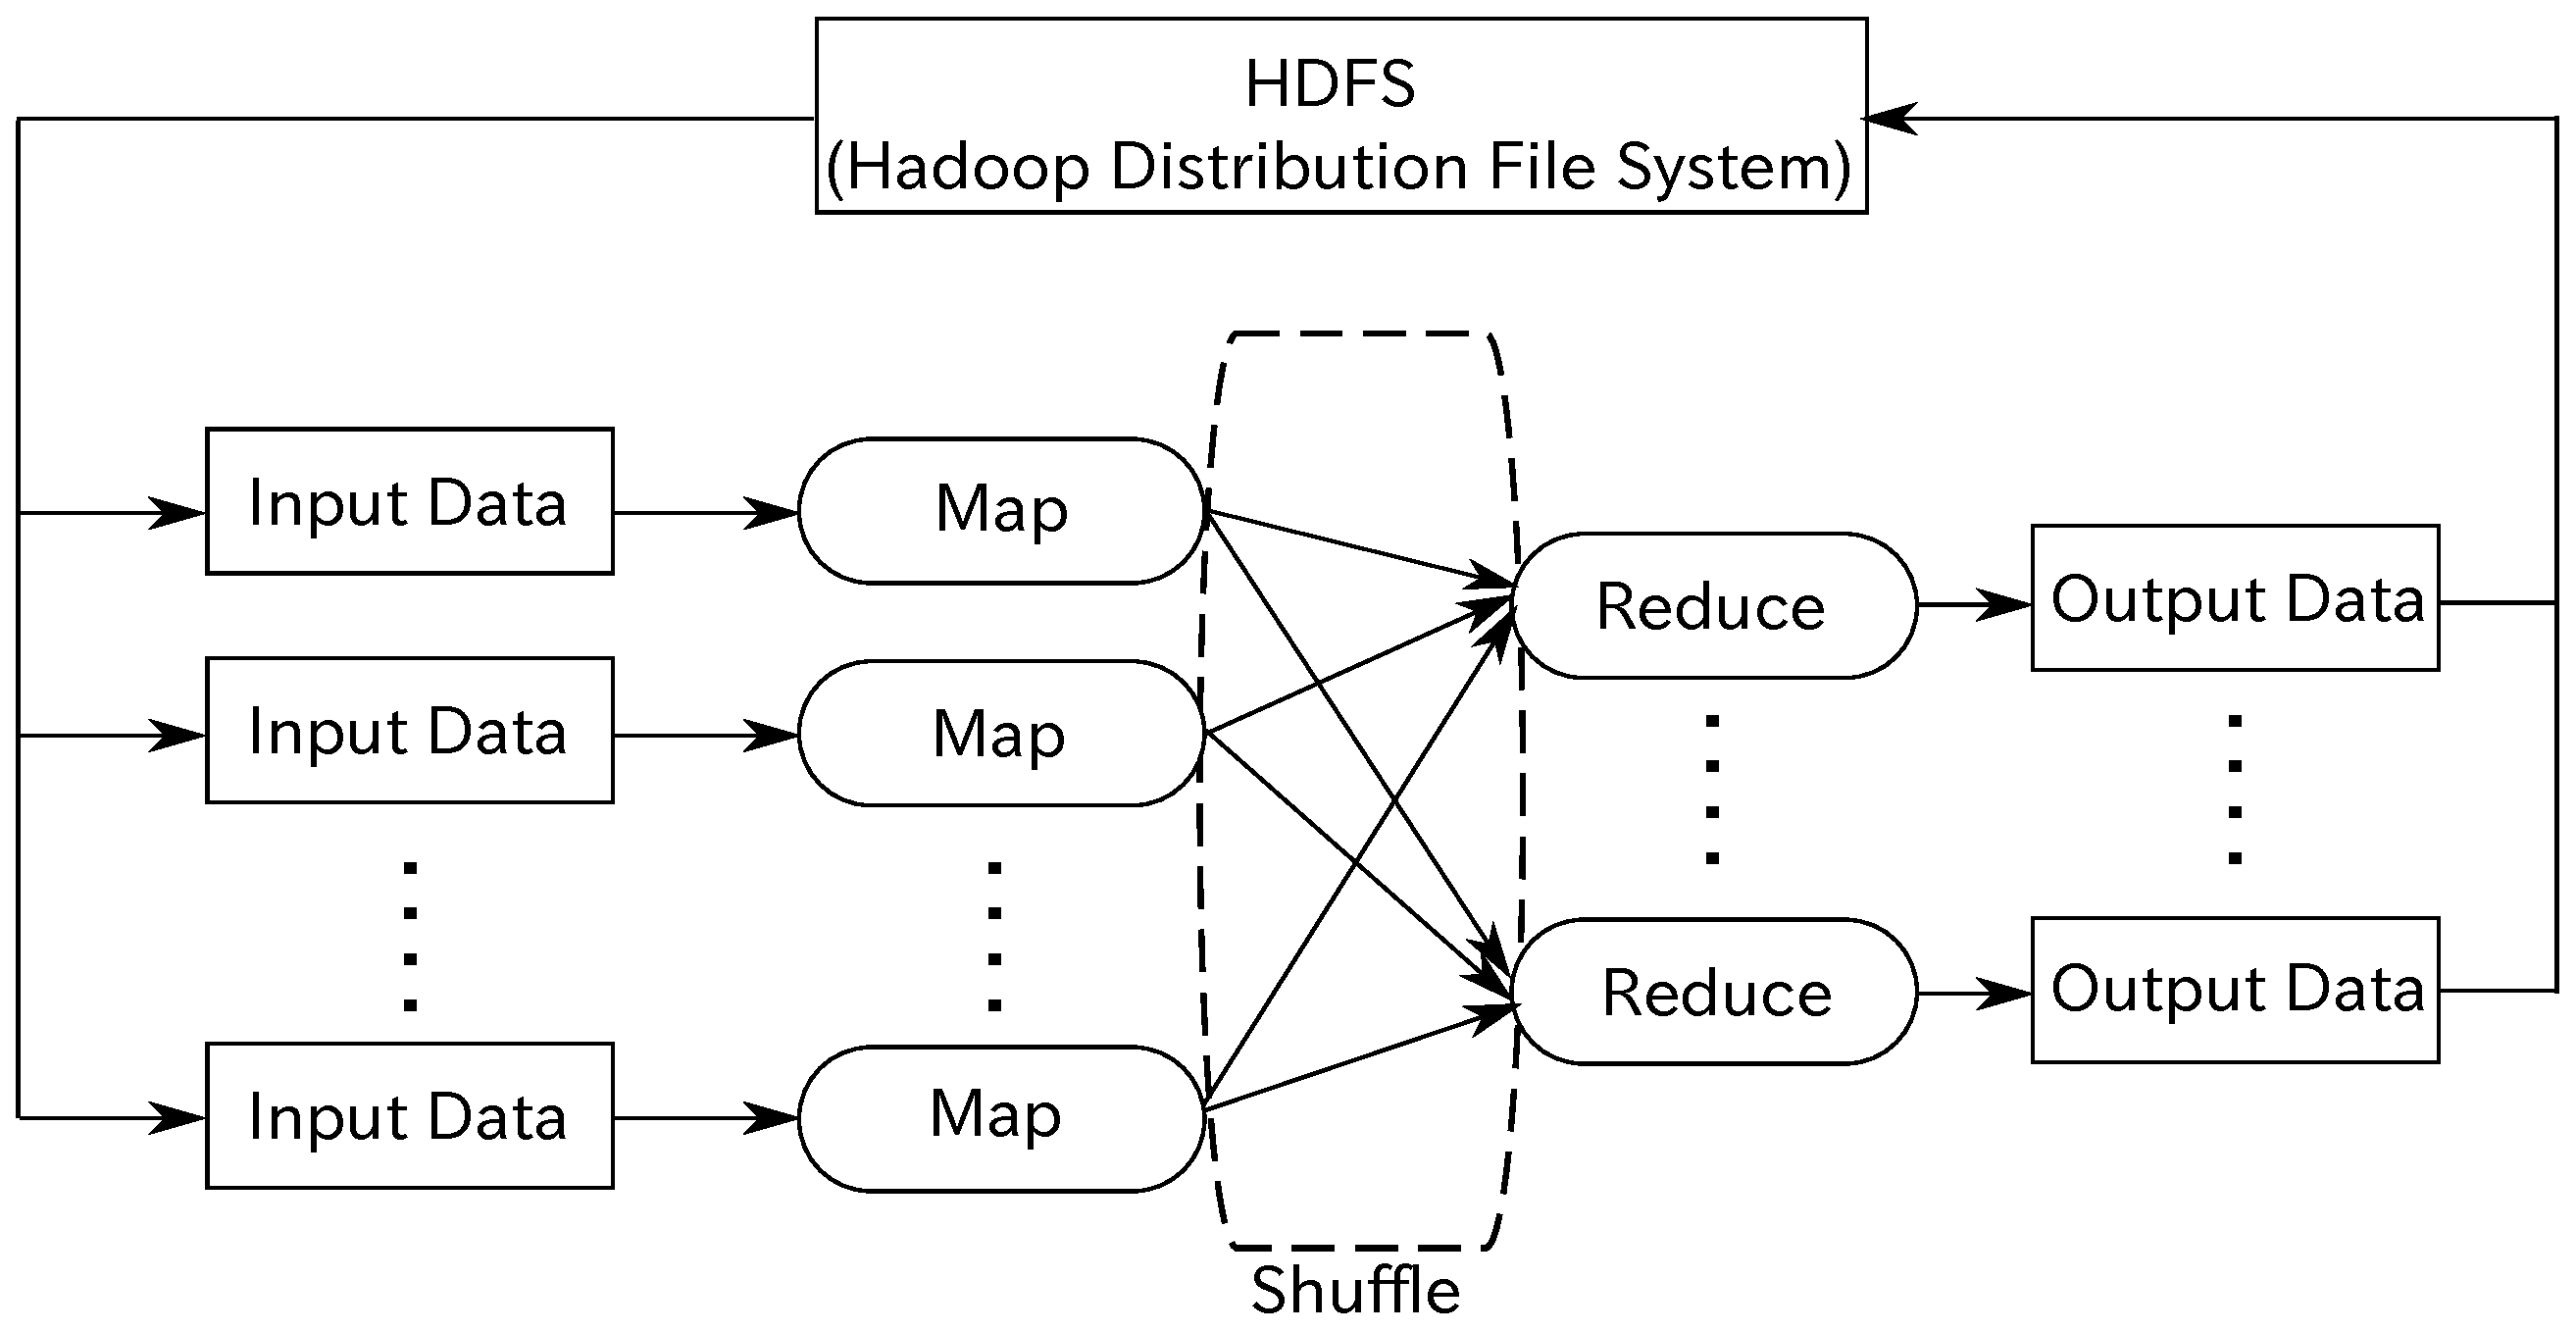
\includegraphics[width=100mm]{fig/MapReduce.eps}
  \caption{Hadoopの分散処理の流れ}
  \label{fig:MapReduce}
 \end{center}
\end{figure}
%
Hadoopは分散並列処理システムであり,Hadoopのみでは機械学習が行えない.し
かし,機械学習するためのライブラリ等のツールがいくつか用意されており,
Hdp2班では,Sparkを用いた.次節にて,Sparkについて簡単に説明する.
%%%%%%%%%%%%%%%%%%%%%%
\subsection{Spark}
%%%%%%%%%%%%%%%%%%%%%%
SparkとはHadoop同様,分散並列処理を可能にするフレームワークである.Spark
自身はHDFSを持っておらず,HadoopのHDFSを利用することが出来る.Hadoopは一
つの処理が終わるたびにHDFSに書き込まなければならないが,Sparkではインメ
モリを用いることで
一つの処理ごとにHDFSに書き込む必要が無く,処理を高速化している.図
\ref{fig:Hadoop_vs_Spark}にHadoopの場合とSparkとHadoopを組み合わせた場合
の処理の流れを示す.図\ref{fig:hs}では,まず,大きなデータを
MapReduce処理で加工し,その後Sparkで分散処理している.図\ref{fig:hs}中の
YARN(Yet Another Resource Negotiator)とは,分散環境でのリソース管理とス
ケジューリングの機能とアプリケーション実行機能の分離することでMapReduce
処理以外にも対応したものである.
%
 \begin{figure}
  \begin{center}
   \subfigure[Hadoopのみ]{%
   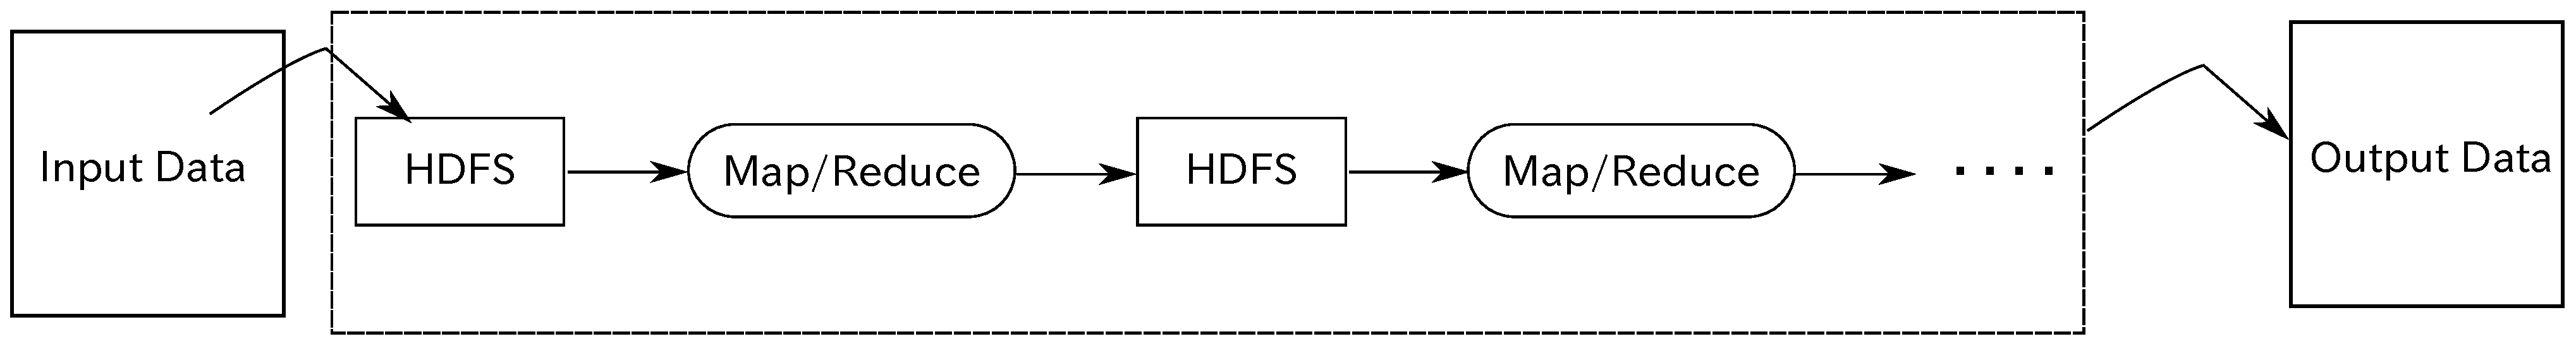
\includegraphics[width=170mm]{fig/Hadoop_d.eps}}%
   \\
   \subfigure[HadoopとSparkの組み合わせ]{\label{fig:hs}
   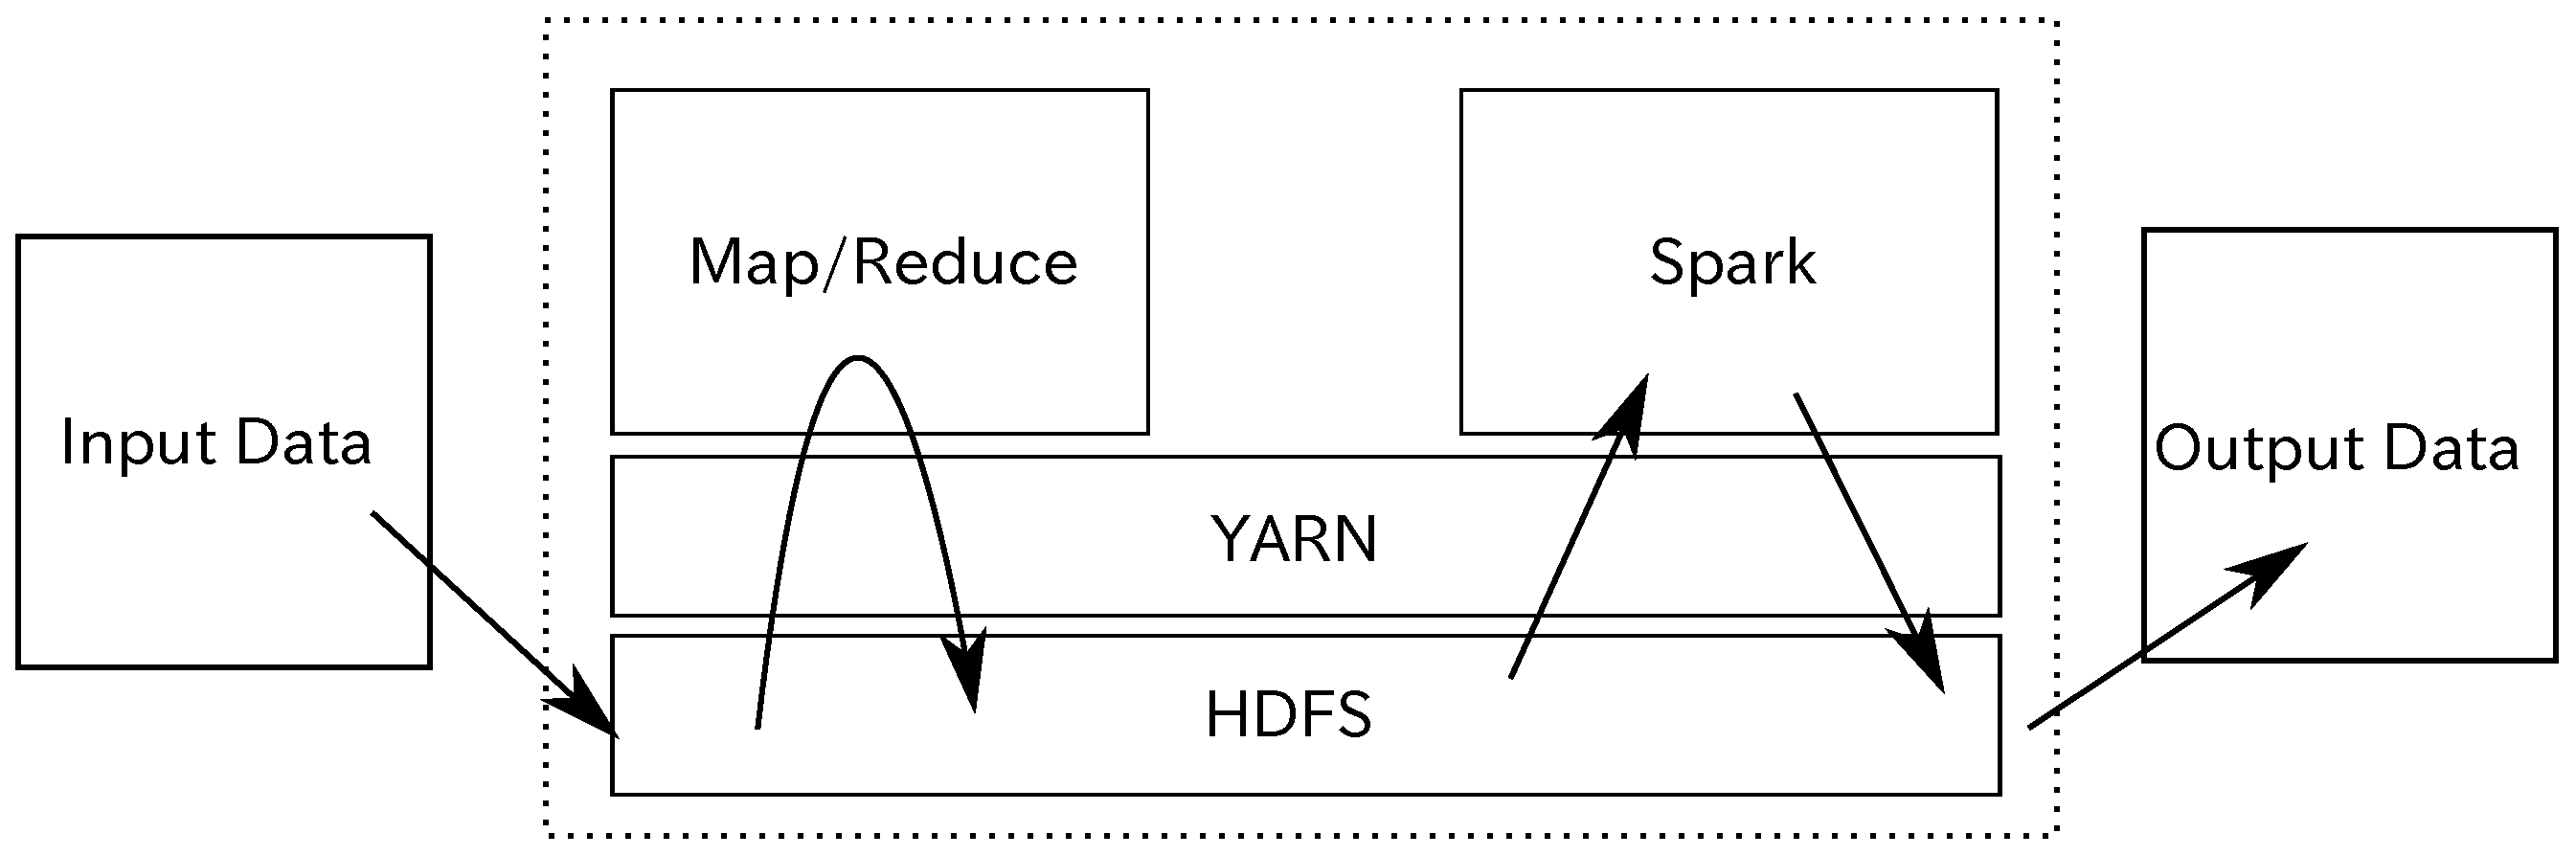
\includegraphics[width=120mm]{fig/Hadoop_spark.eps}}%
  \end{center}
  \caption{HadoopとSpark}
  \label{fig:Hadoop_vs_Spark}
 \end{figure}
%
Sparkのデータ処理にはRDD(Resilient Distributed Dataset)と呼ばれるデータ
構造を用いている.RDDは大量のデータを要素として保持する分散コレクション
である.RDD内はパーティションというかたまりに分割されており,これが分散
処理の単位である.RDDをパーティションごとに複数のPCで分散処理することで
一台のPCでは難しいビッグデータの分散処理が可能となる.
%
\begin{figure}[bp]
 \begin{center}
  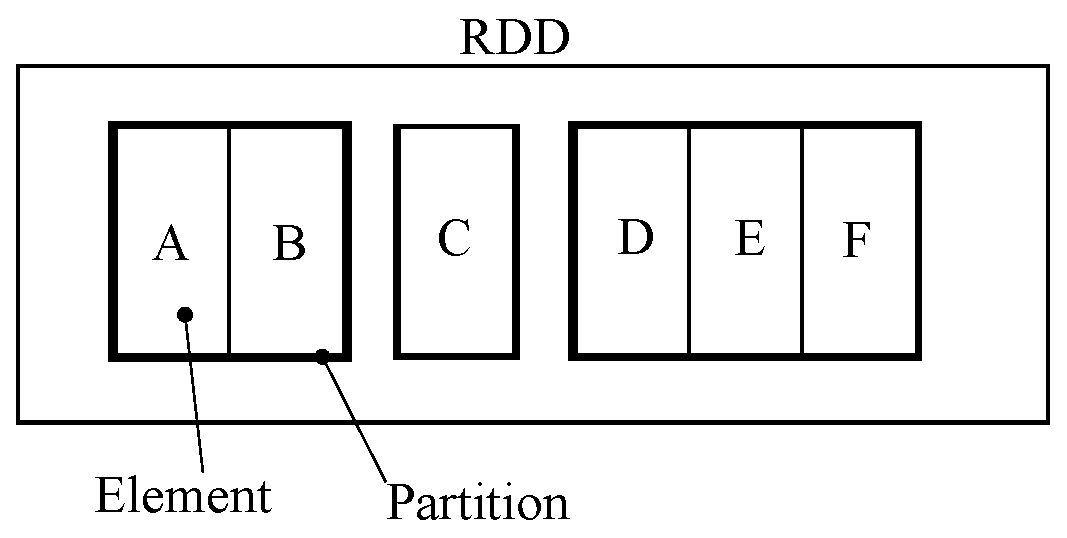
\includegraphics[width=80mm]{fig/RDD.eps}
  \caption{RDDの構造}
  \label{fig:RDD}
 \end{center}
\end{figure}
%
また,Sparkには機械学習用ライブラリMLlibが用意されており,機械学習の分散並列処理が可能
である.なお,使用可能な言語はJava,Python,R言語である.
%%%%%%%%%%%%%%%%%%%%
\subsection{機械学習(Machine Learning)}
%%%%%%%%%%%%%%%%%%%%
本節でHdp2班が行った二つの学習テーマとその内容について簡単に説明する.
%%%%%%%%%%%%%%%%%%%%%%%%%%%%%%%%
\subsubsection{スパムメールの分類}
%%%%%%%%%%%%%%%%%%%%%%%%%%%%%%%%
一つ目の学習テーマとしてスパムメールの分類を行った.データセットとして
Spambase DataSet\cite{Spam}を用いた.
このデータセットは4601通のメールで構成されており,うち1813通のスパムメールと2788通の非スパムメー
ルである.また,57次元のベクトルとして特徴量抽出済みである.
1〜48番目の要素は特定の変数名の出現頻度,49〜54番目の要素は記号文
字の出現頻度,55〜57番目の要素は,大文字の連なりの長さの平均,最長,
合計である.学習アルゴリズムとして,ロジスティック回帰を使用した.
ロジスティック回帰とは,識別関数としてシグモイド関数を用いた回帰モデルであ
る.シグモイド関数は以下の式で表される.また,図\ref{fig:sigmoid}にシグ
モイド関数のグラフを示す.
%
\begin{equation}
 f_\theta (x) = \frac{1}{1+e^{-\theta x}}
\end{equation}
%
\begin{figure}[bp]
 \begin{center}
  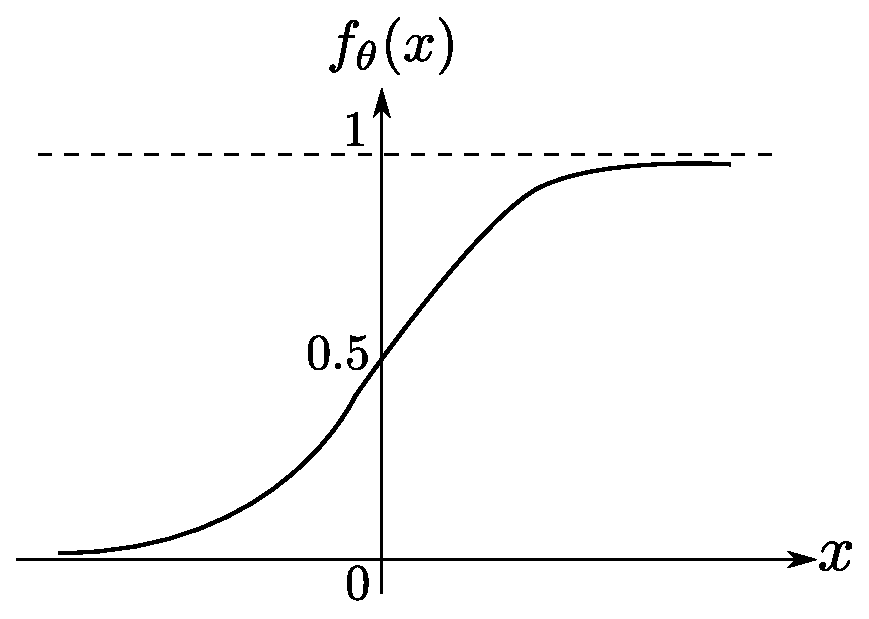
\includegraphics[width=60mm]{fig/sigmoid.eps}
  \caption{シグモイド関数}
  \label{fig:sigmoid}
 \end{center}
\end{figure}
%
ただし,$\theta$はパラメータである.スパム,非スパムを正しく分類できる確
率を最大化するパラメータ$\theta$を決定することが目的である目的関数として
対数尤度関数$\log L(\theta)$を使用し,以下の式
%
\begin{equation}
 \log L(\theta) = \sum^n_{i=1}(y^{(i)}\log f_\theta(x)+(1-y^{(i)})\log
  (1-f_\theta (x)))
\end{equation}
%
を最大化するするようなパラメータ$\theta$を学習(更新)する.パラメータの
更新式を求めるには,最急降下法や確率的勾配法,準ニュートン法などがあるが,
SparkのMLlibで用意されている準ニュートン法を用いてパラメータを更新した.

%%%%%%%%%%%%%%%%%%%%%%%%%%%%%%%%%%%%%%
\subsubsection{画像認識}
%%%%%%%%%%%%%%%%%%%%%%%%%%%%%%%%%%%%%%
二つ目の学習テーマとして画像認識を行った.データセットとしてCIFAR-10\cite{CIFAR}を
用いた.CIFAR-10は60000枚の画像から構成され,うち50000枚が訓練用画
像であり,残り10000枚はテスト用画像である.オープンライブラリの
scikit-imageを用いてHOG特徴量を抽出し,前節と同じくロジスティック回帰で画像認
識(多クラス分類)を行った.HOG特徴量とは,局所領域の勾配ヒストグラムを
特徴ベクトル化したものである.局所的な幾何学変化や照明変化にロバストであ
る利点がある.

%%%%%%%%%%%%%%%%%%%%%%%%
\subsection{実行条件と結果}
%%%%%%%%%%%%%%%%%%%%%%%%
実行条件はスタンドアローンモードではPC一台,完全分散モードではMaster一台,
Slave二台の計三台で行った.なお,OSはすべてUbuntu 14.04 LTSである.
表\ref{tab:mail_result}にスパムメールの検出の結果を示し,表\ref{tab:image_result}に画像
認識の結果を示し,表\ref{tab:time}にそれぞれの実行時間を示す.
チューニングをしたことにより,精度よく学習できた.また,完全分散において
同じプログラムを連続で実行すると実行時間が少なくなることが確認された.
キャッシュによって早くなったと考えられる.それでも完全分
散モードより実行時間が多かった.これはデータセットが小さく,一台のPCで早
く実行できるためであると考えられる.
また,画像認識ではスパムメールの
検出のときに使用したデータセットより大きい(訓練データ約900MB,テストデー
タ約180MB)ものを用いたがそれでもスタンドアローンモードが早かったが,二
つのモードの時間差は小さくなっている.さらにこれより大きいデータセットで
実行すれば完全分散の恩恵を受けることが出来ると考えられる.また,学習結果
を見るとうまく分類が行えていない.つまり,学習が正しくできないことによっ
て,実行時間が増えているとも考えられる.学習アルゴリズム,プログラムの再
検討も必要であると思った.
%
\newpage
\begin{table}[h]
\centering
\caption{スパムメールの検出の結果}
\label{tab:mail_result}
\fontsize{9pt}{10pt}\selectfont
\begin{tabular}{c|c|c|c|c} \hline
非スパム再現率&スパム再現率&非スパム適合率&スパム適合率&AUC(PR) \\\hline \hline 
91.92\% & 90.41\% & 93.48\% & 88.21\% & 0.9123 \\ \hline
\end{tabular}
\end{table}
%
%
\begin{table}[h]
\centering
\caption{画像認識の結果}
 \label{tab:image_result}
\fontsize{8pt}{9pt}\selectfont
 \begin{tabular}{c|c|c|c|c|c|c|c|c|c|c} \hline
  &Airplane&automobile&Bird&Cat&Derr&Dog&Frog&Horse&Ship&Truck \\ \hline
Precision&55.53\% & 64.49\% & 42.98\% & 38.21\%& 42.69\% & 45.91\% & 51.63\% & 57.36\% & 57.91\% & 62.30\% \\ \hline
 Recall&55.70\% & 66.10\% & 35.80\% & 29.80\% &42.90\% & 43.80\% &63.40\% & 60.40\% & 62.20\% & 65.10\%  \\ \hline
\end{tabular}
\end{table}
%
\begin{table}[h]
\centering
\caption{実行時間の比較}
\label{tab:mail_time}
\fontsize{9pt}{10pt}\selectfont
\begin{tabular}{c||c|c} \hline
&スタンドアローン&完全分散 \\\hline \hline 
スパムメールの検出& 5.258[s]& 29.124[s]  \\ \hline
画像認識&25.903[s]& 35.300[s]   \\ \hline
\end{tabular}
\end{table}
%
%%%%%%%%%%%%%%%%%%%
\section{自分の分担範囲}
%%%%%%%%%%%%%%%%%%
機械学習・分散処理(Hadoop,Spark)の理論調査,毎週のレポート作成
%%%%%%%%%%%%%%%%%%%
\section{感想}
%%%%%%%%%%%%%%%%%%
本プロジェクトを通して,ビッグデータの分散並列処理の原理を理解し,実装す
ることができた.また,機械学習の理論を理解し,分散並列処理に適用できた.
本プロジェクト研究で機械学習を勉強し,今流行りのディープラーニングも勉強
してみたいと思った.
\newpage
%%%%%%%%%%%%%%%%%%
\section{評価}
%%%%%%%%%%%%%%%%%%
\begin{table}[hbtp]
\centering
\caption{評価}
\label{tab:評価}
\fontsize{9pt}{10pt}\selectfont
\begin{tabular}{c|c||p{100mm}} \hline
 学籍番号&氏名     &評価   \\ \hline \hline
 16344217&自分& 機械学習の理論を担当した.機械学習や分
		 散処理の理論の方は理解できたが,
		 プログラムの方ではあまり貢献できなかった.また,各メンバーの進捗をま
		 とめ毎回レポートを制作した.\\ \hline
16344201&井上 聖也&Sparkの機械学習プログラムを作ってくれた.理論やプログラム
		 に関して色々助けてもらった.チームリーダーとしてメンバーを統括し
		 プロジェクト研究を速やかに進めることができた.\\ \hline
16344216&田中 良道& HadoopとSparkについて調査してくれた.通信エラー
		 の解決法など色々調査してくれた.\\ \hline 
15344229&沈 歩偉 & Hadoop,Sparkの完全分散処理環境を構築してくれた.実行
		 時間の比較実験などしっかりやってくれた.また,
		 Hadoop,Sparkのインストールに困っている時,手伝ってくれた. \\ \hline
\end{tabular}
\end{table}
%参考文献
\begin{thebibliography}{99}
\addcontentsline{toc}{section}{参考文献}

 \bibitem{Spam} "Spambase Data Set",
		 https://archive.ics.uci.edu/ml/datasets/Spambase, 2016年8月9日最終確認.

 \bibitem{CIFAR} "The CIFAR-10 dataset",
		 https://www.cs.toronto.edu/~kriz/cifar.html, 2016年8月9日最終確認.

\end{thebibliography}

\end{document}
